\begin{figure}[t]
\centering
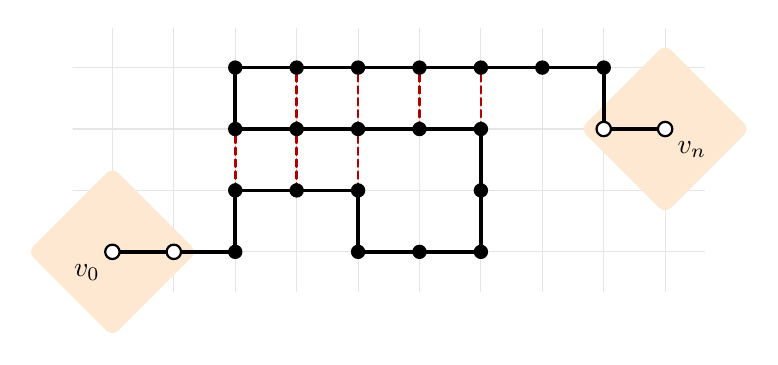
\begin{tikzpicture}[line cap=round]
\draw[black!10,step=0.78] (-0.5,-0.5) grid (7.52,2.84);
\fill[orange!18,rounded corners=3pt] (5.944,1.560) -- (7.020,2.636) -- (8.096,1.560) -- (7.020,0.484) -- cycle;
\fill[orange!18,rounded corners=3pt] (-1.076,0.000) -- (0.000,1.076) -- (1.076,0.000) -- (0.000,-1.076) -- cycle;
\draw[red!70!black,line width=1.0pt,dash pattern=on 2.5pt off 1.8pt] (1.560,0.780) -- (1.560,1.560);
\draw[red!70!black,line width=1.0pt,dash pattern=on 2.5pt off 1.8pt] (2.340,0.780) -- (2.340,1.560);
\draw[red!70!black,line width=1.0pt,dash pattern=on 2.5pt off 1.8pt] (3.120,0.780) -- (3.120,1.560);
\draw[red!70!black,line width=1.0pt,dash pattern=on 2.5pt off 1.8pt] (4.680,1.560) -- (4.680,2.340);
\draw[red!70!black,line width=1.0pt,dash pattern=on 2.5pt off 1.8pt] (3.900,1.560) -- (3.900,2.340);
\draw[red!70!black,line width=1.0pt,dash pattern=on 2.5pt off 1.8pt] (3.120,1.560) -- (3.120,2.340);
\draw[red!70!black,line width=1.0pt,dash pattern=on 2.5pt off 1.8pt] (2.340,1.560) -- (2.340,2.340);
\draw[black,line width=1.3pt] (0.000,0.000) -- (0.780,0.000);
\draw[black,line width=1.3pt] (0.780,0.000) -- (1.560,0.000);
\draw[black,line width=1.3pt] (1.560,0.000) -- (1.560,0.780);
\draw[black,line width=1.3pt] (1.560,0.780) -- (2.340,0.780);
\draw[black,line width=1.3pt] (2.340,0.780) -- (3.120,0.780);
\draw[black,line width=1.3pt] (3.120,0.780) -- (3.120,0.000);
\draw[black,line width=1.3pt] (3.120,0.000) -- (3.900,0.000);
\draw[black,line width=1.3pt] (3.900,0.000) -- (4.680,0.000);
\draw[black,line width=1.3pt] (4.680,0.000) -- (4.680,0.780);
\draw[black,line width=1.3pt] (4.680,0.780) -- (4.680,1.560);
\draw[black,line width=1.3pt] (4.680,1.560) -- (3.900,1.560);
\draw[black,line width=1.3pt] (3.900,1.560) -- (3.120,1.560);
\draw[black,line width=1.3pt] (3.120,1.560) -- (2.340,1.560);
\draw[black,line width=1.3pt] (2.340,1.560) -- (1.560,1.560);
\draw[black,line width=1.3pt] (1.560,1.560) -- (1.560,2.340);
\draw[black,line width=1.3pt] (1.560,2.340) -- (2.340,2.340);
\draw[black,line width=1.3pt] (2.340,2.340) -- (3.120,2.340);
\draw[black,line width=1.3pt] (3.120,2.340) -- (3.900,2.340);
\draw[black,line width=1.3pt] (3.900,2.340) -- (4.680,2.340);
\draw[black,line width=1.3pt] (4.680,2.340) -- (5.460,2.340);
\draw[black,line width=1.3pt] (5.460,2.340) -- (6.240,2.340);
\draw[black,line width=1.3pt] (6.240,2.340) -- (6.240,1.560);
\draw[black,line width=1.3pt] (6.240,1.560) -- (7.020,1.560);
\filldraw[fill=white,draw=black,line width=0.8pt] (0.000,0.000) circle (2.6pt);
\filldraw[fill=white,draw=black,line width=0.8pt] (0.780,0.000) circle (2.6pt);
\fill[black] (1.560,0.000) circle (2.6pt);
\fill[black] (1.560,0.780) circle (2.6pt);
\fill[black] (2.340,0.780) circle (2.6pt);
\fill[black] (3.120,0.780) circle (2.6pt);
\fill[black] (3.120,0.000) circle (2.6pt);
\fill[black] (3.900,0.000) circle (2.6pt);
\fill[black] (4.680,0.000) circle (2.6pt);
\fill[black] (4.680,0.780) circle (2.6pt);
\fill[black] (4.680,1.560) circle (2.6pt);
\fill[black] (3.900,1.560) circle (2.6pt);
\fill[black] (3.120,1.560) circle (2.6pt);
\fill[black] (2.340,1.560) circle (2.6pt);
\fill[black] (1.560,1.560) circle (2.6pt);
\fill[black] (1.560,2.340) circle (2.6pt);
\fill[black] (2.340,2.340) circle (2.6pt);
\fill[black] (3.120,2.340) circle (2.6pt);
\fill[black] (3.900,2.340) circle (2.6pt);
\fill[black] (4.680,2.340) circle (2.6pt);
\fill[black] (5.460,2.340) circle (2.6pt);
\fill[black] (6.240,2.340) circle (2.6pt);
\filldraw[fill=white,draw=black,line width=0.8pt] (6.240,1.560) circle (2.6pt);
\filldraw[fill=white,draw=black,line width=0.8pt] (7.020,1.560) circle (2.6pt);
\node[below left=1pt] at (0.000,0.000) {$v_0$};
\node[below right=1pt] at (7.020,1.560) {$v_n$};
\end{tikzpicture}
\caption{A path (solid) with its 7 chords (dashed), drawn in a plane for illustration; on $\T_L$ chords may also point out of the plane or across the periodic identification. Open circles are the uncharged vertices: the endpoints and their lattice neighbours on the path (shaded). Every induced bond at a charged vertex (black) has two interior endpoints, so the local inequalities (A1)--(A2) apply to it.}
\label{fig:path}
\end{figure}
